% 2008 年上海卷理科第 15 题：圆 Ω 与 x、y 轴正半轴分别切于 C、D，
%   A、B、C、D 为圆的四等分点（A 上、B 右、C 下、D 左）。
% 来源 PDF：gaokaomath-src/普通高考/2008/2008上海理.pdf
% SHA-256：df3f761eb2551cc795c0efb1c90c284a54b95265e327f21abb60aa0f4bdd86a2
% 原页：2008上海理.pdf 第 1 页（A3 三栏）第 2 栏，书页码 479。
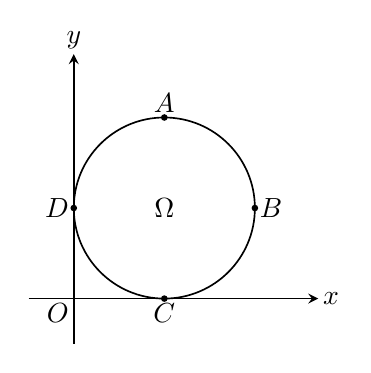
\begin{tikzpicture}[x=1.15cm, y=1.15cm, semithick,
  every node/.style={inner sep=1.5pt}]
  \draw[->,>=stealth] (-0.5,0) -- (2.7,0) node[right] {$x$};
  \draw[->,>=stealth] (0,-0.5) -- (0,2.7) node[above] {$y$};
  \node[below left] at (0,0) {$O$};
  \draw (1,1) circle (1);
  \node at (1,1) {$\Omega$};
  \fill (1,2) circle (1.2pt); \node[above] at (1,2) {$A$};
  \fill (2,1) circle (1.2pt); \node[right] at (2,1) {$B$};
  \fill (1,0) circle (1.2pt); \node[below] at (1,0) {$C$};
  \fill (0,1) circle (1.2pt); \node[left] at (0,1) {$D$};
\end{tikzpicture}
